%(BEGIN_QUESTION)
% Copyright 2009, Tony R. Kuphaldt, released under the Creative Commons Attribution License (v 1.0)
% This means you may do almost anything with this work of mine, so long as you give me proper credit

An NDIR gas analyzer is going to be used to measure the concentration of nitrous oxide (N$_{2}$O) in the presence of methane (CH$_{4}$).  The infrared absorption characteristics for these gases are shown in the following plot (methane in blue; nitrous oxide in red):

$$\includegraphics[width=15.5cm]{i04174x01.eps}$$

Identify which gases the ``reference cell'' and ``detector'' chambers should be filled with, and whether or not this analyzer will require filter cells.  If filter cells are required, identify the gas(es) they should be filled with as well.

\vskip 20pt \vbox{\hrule \hbox{\strut \vrule{} {\bf Suggestions for Socratic discussion} \vrule} \hrule}

\begin{itemize}
\item{} Is there any reason the analyzer cannot be configured to measure the concentration of methane, with nitrous oxide as the interferent?
\item{} Supposing CH$_{4}$ and N$_{2}$O are the only gases present in this process stream to any significant degree, are there alternative analyzer technologies you might suggest for the application?
\end{itemize}

\underbar{file i04174}
%(END_QUESTION)





%(BEGIN_ANSWER)

\noindent
{\bf Partial answer:}

\vskip 10pt

Filter cells {\it are required} for this NDIR analyzer!

%(END_ANSWER)





%(BEGIN_NOTES)

Fill the detector chambers with nitrous oxide (N$_{2}$O) gas.  Fill the reference cell with any non-absorbing gas (e.g. nitrogen).  Fill the filter cells with methane (CH$_{4}$) gas.

%INDEX% Measurement, analytical: nondispersive optical

%(END_NOTES)


